\chapter{研究现状}\label{chapter:relatedwork}
本章第一节首先对数据模型和要解决的查询问题进行了定义,然后从以下三方面介绍了相关的研究工作:轨迹数据管理、轨迹压缩、轨迹距离度量和$k$近邻轨迹查询,最后对本章内容进行小结。

\section{数据模型及问题定义}\label{chapter-related-coll}
本文的研究目标是给定一条查询轨迹,从存储在若干彼此独立的远程结点中的轨迹中找出$k$条距离最短或相似度最高的轨迹。为此,本节首先介绍了轨迹数据模型,接着形式化给出查询定义。

\subsection{轨迹数据}
轨迹是描述移动对象移动行为的数据。通常来说,一条轨迹$T$可看做包含$n$个元素(即轨迹点)的时间序列。每个轨迹点$\vp$包含了时间、位置等维度的信息。因此轨迹可被形式化定义为如下:
\begin{define}[轨迹(Trajectory)]
轨迹形式化表示为:$T=\{\bp_{0}, \bp_{1},\cdots, \bp_{n-1}\}$。
\begin{equation}
T=\{\bp_{0}, \bp_{1},\cdots, \bp_{n-1}\}
\end{equation}
其中$|T|=n$代表轨迹所包含的点数,即轨迹的长度。每个轨迹点$\bp$包含时间($t$)、位置($l$)等维度的信息。因而$|\bp|=d$称为轨迹的维度。此外轨迹中的点严格按时间升序排列,即$\forall i,j,0\le i\le j < n$则$\bp_{i}.t \le \bp_{j}.t$。
\end{define}

轨迹数据的来源多样且复杂。根据移动对象的划分可分为如下几类\cite{GQSurvery}:
\begin{itemize}
	\item \textsf{人类活动轨迹数据:}该类数据分为主动式和被动式。主动式数据是人们主动利用移动定位设备分享或汇报自己的位置等信息。典型的有社交网络中的数据,用户提交位置获得服务的数据。被动式数据是人们无意间使用各种服务时所产生的轨迹数据。典型的有公交刷卡轨迹\cite{WYL}和手机的信令轨迹数据\cite{zzgSF}。

	\item \textsf{交通工具轨迹数据:}这类数据主要是交通工具使用车载GPS设备所产生的移动轨迹数据。例如,出租车、公交车的活动轨迹数据\cite{DTKST}。
	
	\item \textsf{动物活动轨迹数据:}这类数据是为了研究动物生活、迁徙等行为和习惯而捕获的数据\cite{LeeHW07}
	\footnote{http://www.fs.fed.us/pnw/starkey/data/tables/}。
	
		\item \textsf{自然现象活动轨迹数据:}这类数据典型的有台风、冰山、海洋事件等的轨迹数据\footnote{http://weather.unisys.com/hurricane/atlantic/},用以探索自然现象的活动规律。
\end{itemize}

轨迹数据符合大数据时代的 3V 特征,即量大、实时、多样。但是由于受设备、采样频率等因素影响,数据质量较低且各个轨迹的采样间隔差异显著。
这些问题导致原始轨迹数据的可用性较低。这为我们对其管理和有效利用造成了挑战。

\subsection{分布式$k$近邻轨迹查询}
轨迹数据往往是分布式采集并存储的。为此假设有$M$个远程结点,每个远程结点$i$包含轨迹数据集${\cal D}_{i}$。那么整个分布式轨迹数据集${\cal D}=\bigcup_{i=1}^{M} {\cal D}_{i}$。我们的目标是给定查询轨迹,从分布式轨迹数据集${\cal D}$中,找出与其距离最近的$k$条轨迹。下面我们将给出查询的形式化定义:
\begin{define}[分布式k近邻轨迹查询]
	该查询形式为kNN$({\cal Q}, {\cal D},DM,k)$,其中$\cal Q$为给定查询轨迹,${\cal D}$为分布式轨迹数据集, $DM$为距离度量准则以及$k$为返回结果集大小。查询的目标是返回满足如下条件的轨迹集$\cal S$:(1)${\cal S} \subseteq {\cal D}$;(2)$| {\cal S}|=k$;
	(3)$\forall {\cal C} \in {\cal S}, {\cal C}' \in {{\cal D} - \cal S}$,$DM({\cal Q},{\cal C}) \le DM({\cal Q},{\cal C}')$。
\end{define}

与传统的集中式环境下$k$近邻轨迹查询相比,分布式场景下的查询不仅注重查询效率,而且尤其注重通信开销。这是由于分布式场景中,远程结点和协调者结点的带宽资源往往是有限的。而高的通信开销,意味着用户可能要花费更多的金钱。为此,我们应该在不牺牲太多计算开销的基础上降低通信开销。

\section{轨迹数据管理}
本节将介绍如何对轨迹数据进行有效的管理,并介绍现有的轨迹管理系统。

\subsection{轨迹索引}
一个轨迹数据库需要能够在任意数据量下对提供对轨迹的有效查询,而选用合适的轨迹索引策略往往很查询效率有着很大的影响。不同与其他类型数据库,轨迹数据库由于其时间和空间维度特性,需要专门的索引技术,以满足轨迹查询的需求。

现有的轨迹索引技术大致可以分为三类:第一类,使用传统多维索引技术如R树增加时间维度后的改进索引,典型的有三维R树和STR树\cite{PfoserJT00};第二类就是多版本结构的索引,典型的有RT树\cite{Xu1990Rt}、HR树\cite{NascimentoS98}、HR+树\cite{TaoP01}和MV3R树\cite{PapadiasT01}。这类方法为每个时间戳构建一个单独的R树并为两颗连续的树共享共同的部分以减少冗余;第三类就是讲空间维度进行划分得到一系列的方格,然后为每个方格内的数据在时间维度构建索引。这类工作包含SETI\cite{ChakkaEP03}和MTSB树\cite{ZhouZSCK05}。这些算法大都针对静态轨迹数据设计,无法支持轨迹数据动态增加的需求。为此,SEB树\cite{SongR03}和QU-Trade两颗R树的改进以提供数据动态增加。


\subsection{集中式轨迹数据管理}
目前已经有一些针对历史数据的轨迹管理系统以支持轨迹查询\cite{BoteaMNS08,ChakkaEP03,Cudre-MaurouxWM10}。
Botea等首先构建了针对轨迹数据的管理系统PIST\cite{BoteaMNS08}。该系统将轨迹数据以点为基本单位构建空间索引。它首先统计轨迹数据在空间维度的分布,然后构建空间索引划分数据点。最后对每个划分内部的数据根据时间维度构建索引。
Chakka等提出了以子轨迹为基本单元的管理系统SETI\cite{ChakkaEP03}。该系统同样首先根据统计数据构建空间索引。然后根据空间索引划分轨迹数据,并将每个划分内同一移动对象的子轨迹作为基本处理单元构建时空索引。
该工作表明,基于子轨迹的索引策略比基于点的策略查询效率要高。进一步地,Philippe等提出了基于I/O开销模型的轨迹数据管理系统TrajStore以支持动态轨迹划分\cite{Cudre-MaurouxWM10}。此外,TrajStore对每个划分内的子轨迹进行聚类并用簇中心来代表簇内所有轨迹,从而降低数据的存储开销。它还使用了多种数据压缩技术以进一步降低存储开销。Wang等提出针对大内存服务器的轨迹数据系统SharkDB\cite{WangZZS15,WangZXZZS14,ZhengWZSLS18}。该系统提出了3种存储框架用以在降低数据存储开销同时增大内存命中率。此外,它还引入了分层索引以提高查询效率。
上述轨迹系统需进行功能扩展以实现近邻轨迹查询。

\subsection{基于集群的分布式轨迹数据管理}

近10年来,随着Hadoop\footnote{http://hadoop.apache.org/}、OpenStack\footnote{https://www.openstack.org/}和Spark\footnote{http://spark.apache.org/}
等开源大数据处理系统的普及,在这些系统上构建轨迹数据管理分析系统成为新的方向。目前,已经出现了大量基于这些开源分布式平台的轨迹数据管理系统以支持轨迹查询。
Lu等设计了并行的空间数据DBMS系统Parallel-Secondo\cite{LuG12}。该系统在每台节点上使用传统的空间DBMS来实现数据存储和查询实现,仅使用Hadoop作为结点间任务调度器。
Ma等首先提出了基于Hadoop的轨迹数据管理系统\cite{MaYQZ09,YangMQZ09}。为提高查询效率,其构建了两类索引。第一类是基于空间的索引,用于将数据按空间维度划分。此类索引能加速带有空间约束的查询,但如果查询某个移动对象的轨迹,则需要遍历许多数据分区。为此设计了第二类基于移动对象的倒排索引,该索引中存储了每个移动对象的轨迹数据是存储在哪些数据分区上。Clost\cite{TanLN12}系统通过建立一个多层索引用以数据划分。同时,其支持数据的批量增加。
SpatialHaddop\cite{SpatialHadoop}系统是基于Hadoop的典型空间数据管理系统。该系统从以下四个方面对Hadoop进行了改进以满足空间数据查询的需求。
(1)提供了基于多种索引树的存储策略。首先根据全局索引用以完成数据划分,其次在每个数据块内支持块内局部空间索引。这种全局-局部的索引方式能大大减少I/O开销;(2)设计了新的文件读写方式,以支持对块内索引数据的读写;(3)设计了多种查询接口,以方便开发这进行查询调用;(4)设计了基于Pig Latin的查询语言,以方便普通用户实现查询功能。但SpatialHadoop只能用来管理静态数据,当新的数据到达时,需要将整个数据集重新划分,因而开销较大。
AQWA\cite{AlyMHAOEQ15}系统是其改进版本,允许数据动态添加。AQWA建立了新的数据划分模型,同时考虑了用户查询和数据分布对划分的影响。以上系统最终将查询需求,变成定制的Map/Reduce\cite{DeanG04,mapreduce}任务。


此外,还有一些基于Hadoop组件或类Hadoop系统的时空数据管理系统。Ablimit等等提出了基于Hive\footnote{https://hive.apache.org/}的轨迹管理仓库Hadoop-Gis\cite{AjiWVLL0S13},其通过网格索引以提高范围和join查询的效率。MD-HBase\cite{MDHBase}和R-HBase\cite{RHBase}是两个基于HBase\footnote{https://hbase.apache.org/}设计的实时时空数据管理系统。MD-HBase使用Z-Curve空间填充曲线来划分数据空间。接着对所用划分子空间使用四叉树或k-d树索引来构建空间索引。R-HBase使用了局部性更好的希尔伯特空间填充曲线来划分数据空间,并使用R树来构建空间索引。这两个系统借助了HBase的特性可支持数据的实时插入和修改。Geomesa系统\cite{Geomesa}与以上两个系统类似,可以快速部署到类似HBase的键值对存储系统中,且其从语言层定义了空间查询操作接口以方便用户调用。相较于以上系统,Elite系统\cite{XieMCDJ16}专门设计用于处理不确定轨迹数据并提供了丰富的不确定查询接口。

尽管基于Hadoop生态圈内系统构建的分布式轨迹管理系统能满足轨迹查询的需求,但也面临着由于I/O开销较大,无法提供实时、高吞吐率查询服务的问题。为此,出现了许多基于Spark等分布式内存的时空数据管理系统。
SpatialSpark\cite{SpatialSpark}、GeoSpark\cite{GeoSpark}和LocationSpark\cite{Locationspark}是最早的几个空间查询系统,但这些系统仅能处理空间维度上的查询,没有考虑时间维度的影响。
%是最早的两个基于Spark设计的专门用来处理空间数据查询的系统。其中SpatialSpark专门用来处理空间join查询。 GeoSpark设计了一个新的数据结构SRDD用来表示分布式空间数据。SRDD使用全局空间索引来划分数据,且支持每个分区内部构建局部索引。进一步地, LocationSpark\cite{Locationspark} 提出了使用布隆过滤器来 解决数据分布倾斜问题。
最新地,Dong等人提出了新的基于SparkSQL的多维数据管理系统Simba \cite{Simba}。并从查询解析到查询执行等方面作了优化。其中最显著的是在其查询执行计划设计方面使用了空间索引等技术来提高查询效率。此外,它还从语言层提供了用户查询接口。相比以上系统,TrajSpark\cite{TrajSpark}是专门设计用来处理轨迹数据的系统。其实现了3类典型的轨迹查询接口,并利用全局-局部索引策略以提高查询效率。
此外,目前还存在着专门用于对时空数据进行复杂分析的系统\cite{OceanST,STORM}。STORM\cite{STORM}系统设计用来处理交互式近似查询。相比于已有的设计用来精确查找的系统,该系统能在查询提出后,通过逐渐增加采样数据以不断以一定置信度给出查询结果。用户根据系统不断精细的结果随时可以停止查询。OceanST\cite{OceanST}系统同样适用采样技术来获得查询近似结果,且能处理数据不断增加的场景(STORM仅能处理静态历史数据)。此外,它还提供了丰富的查询接口用以满足各种查询需求。


\section{轨迹压缩}\label{sec-c2-reduction}
%\begin{figure}[t]
%	\centering
%	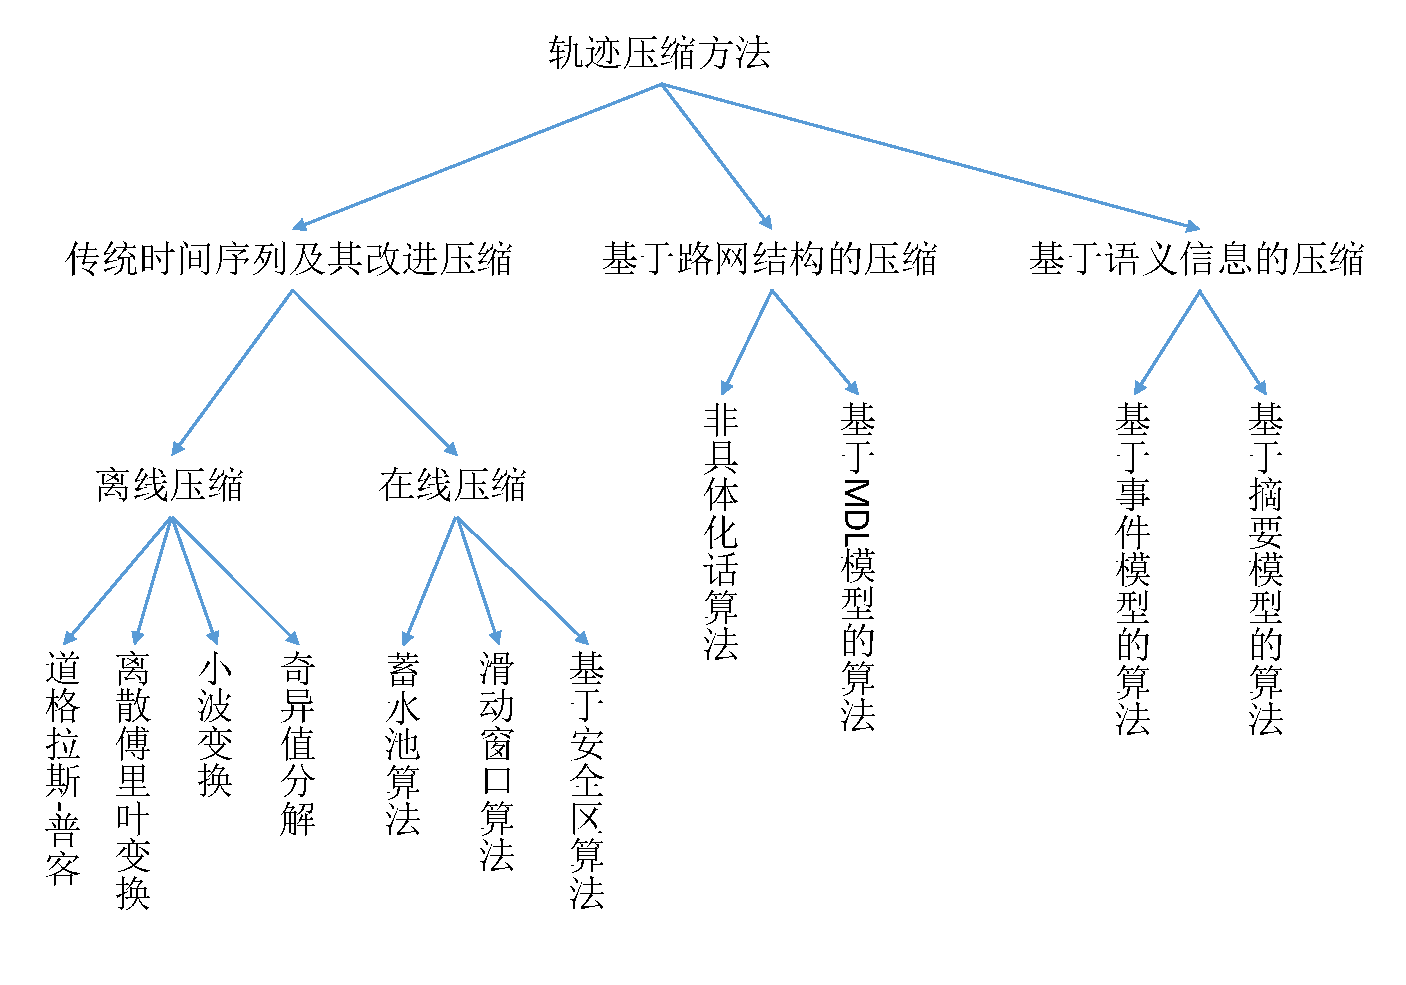
\includegraphics[width=0.73\textwidth]{Fig/chapter2/Compress}
%	\caption{常用轨迹压缩算法}
%	\label{fig-chapter2-compress}
%\end{figure}

将查询轨迹数据压缩是降低通信开销的有效方式。现有轨迹压缩的方法根据处理数据类型的不同可分为3类\cite{jiang}:第一类是传统的时间序列压缩算法,其根据应用场景又可以分为离线和在线压缩两类算法。第二类是基于路网结构的轨迹压缩算法,该类算法依赖于所给路网数据。第三类是语义压缩,其目标是将原始数值型轨迹数据转换为人们能理解的语义信息。下面将详细介绍这三类压缩算法。


\subsection{传统离线时间序列压缩算法}
离线轨迹压缩算法主要的应用场景是,给定一静态历史轨迹数据库,对其中的轨迹进行压缩。该类压缩算法不考虑数据集的增加、删除和修改。
该类算法的提出主要是为了解决时间序列数据的降维(即降低序列的长度)。由于轨迹本质上也是时间序列数据,因此该类方法也可用于轨迹的压缩。尽管相比于传统时间序列数据,轨迹数据属于多维数据。但其各属性维度上数据一般互相独立,因此只需将降维方法应用到各个维度上分别进行压缩即可。本小节主要介绍几种典型的离线时间序列压缩算法。

\textbf{道格拉斯-普克算法:}
道格拉斯-普克(Douglas-Peucker, DP) 算法将原始时间序列看作一条多维曲线,其目标是找出一条与原始曲线相似但使用更少点构成的简化曲线。此外,构成简化曲线的点必须来自原来曲线。
该算法中原始轨迹与简化轨迹间的“不相似性”是通过两条曲线间的豪斯多夫(Hausdorff)距离表示。简化曲线中的点即为压缩后的数据。
%道格拉斯-普克算法的过程由如下5个步骤构成:(1)在曲线首尾两点A,B之间连接一条直线AB;(2)找出曲线上离该直线段距离最大的点C,计算其与AB的距离;(3)比较该距离与预先给定的阈值的大小,如果小于阈值,则该直线段作为曲线的近似,该段曲线处理完毕;(4)如果距离大于阈值,则用C将曲线分为两段AC和BC,并分别对两段取信进行1至3步的处理;(5)当所有曲线都处理完毕时,保留依次收集分割点,得到压缩后的点集。
DP算法的思想简单且性能较好,在各个领域都有广泛的应用。但其缺点就是算法复杂度较高达到$O(n^2)$,$n$是轨迹长度。文献\cite{DPSpeeding}提出了借助外部存储结构的改进算法,把时间复杂度降低为$O(n\log n)$。此外,文献\cite{MeratniaB04}和\cite{LiuZSSKJ15}分别提出了同时时间和空间维度的改进距离函数( Time-Distance Ratio, TDR)和(Top-Down Time Ratio, TD-TR),克服了原始DP算法仅考虑空间维度的缺点。

%\begin{figure} [t]
%	\centering
%	\subfigure[压缩前后数据]{
%		\label{fig:comp}
%		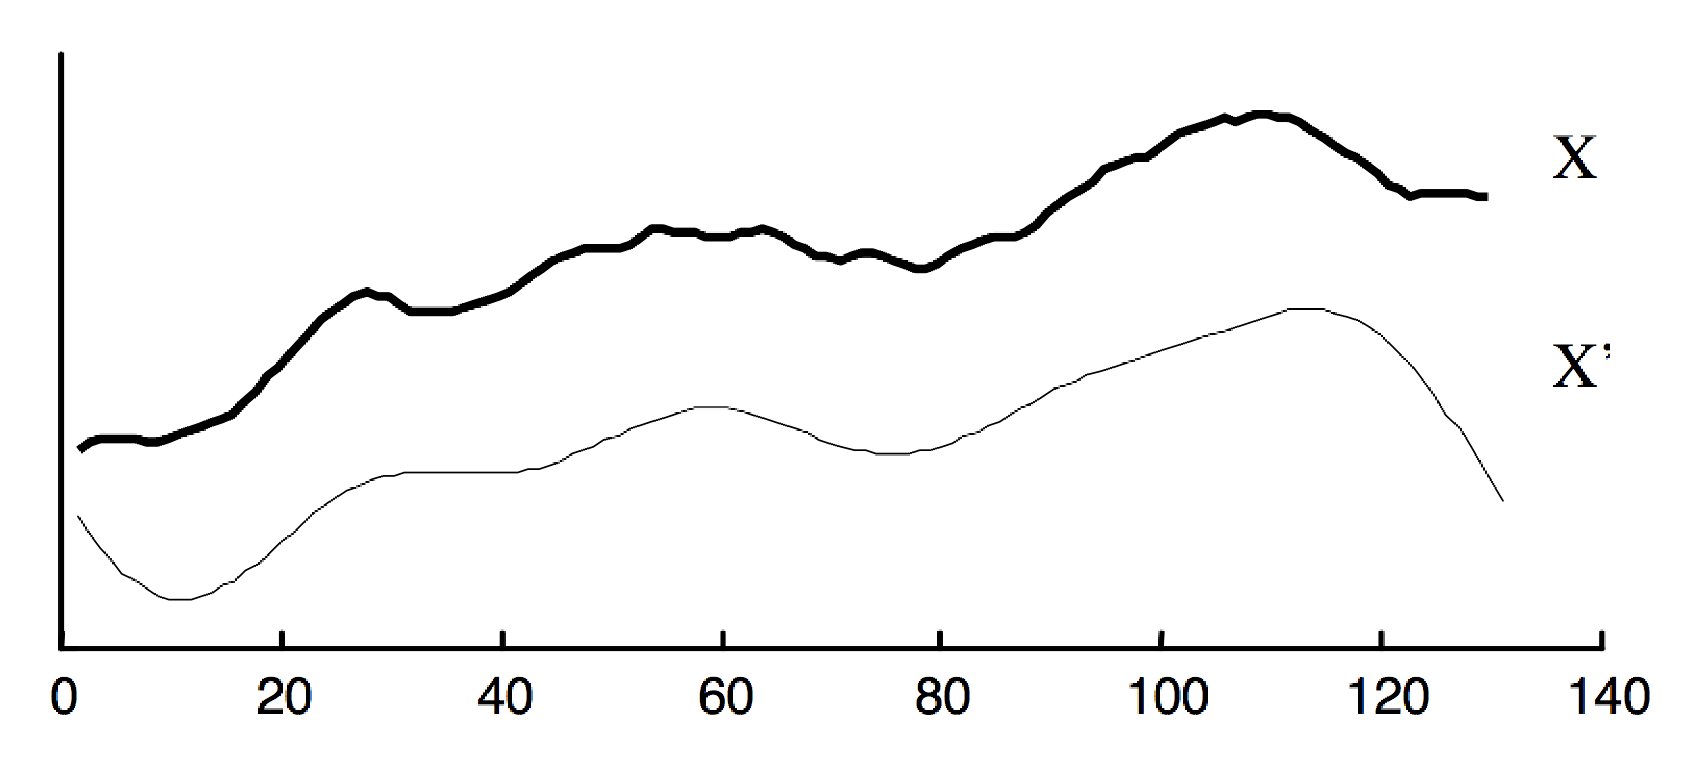
\includegraphics[width=0.45\textwidth]{Fig/chapter2/signal.eps}		
%	}
%	\subfigure[DFT系数]{
%		\label{fig:coefficietns}
%		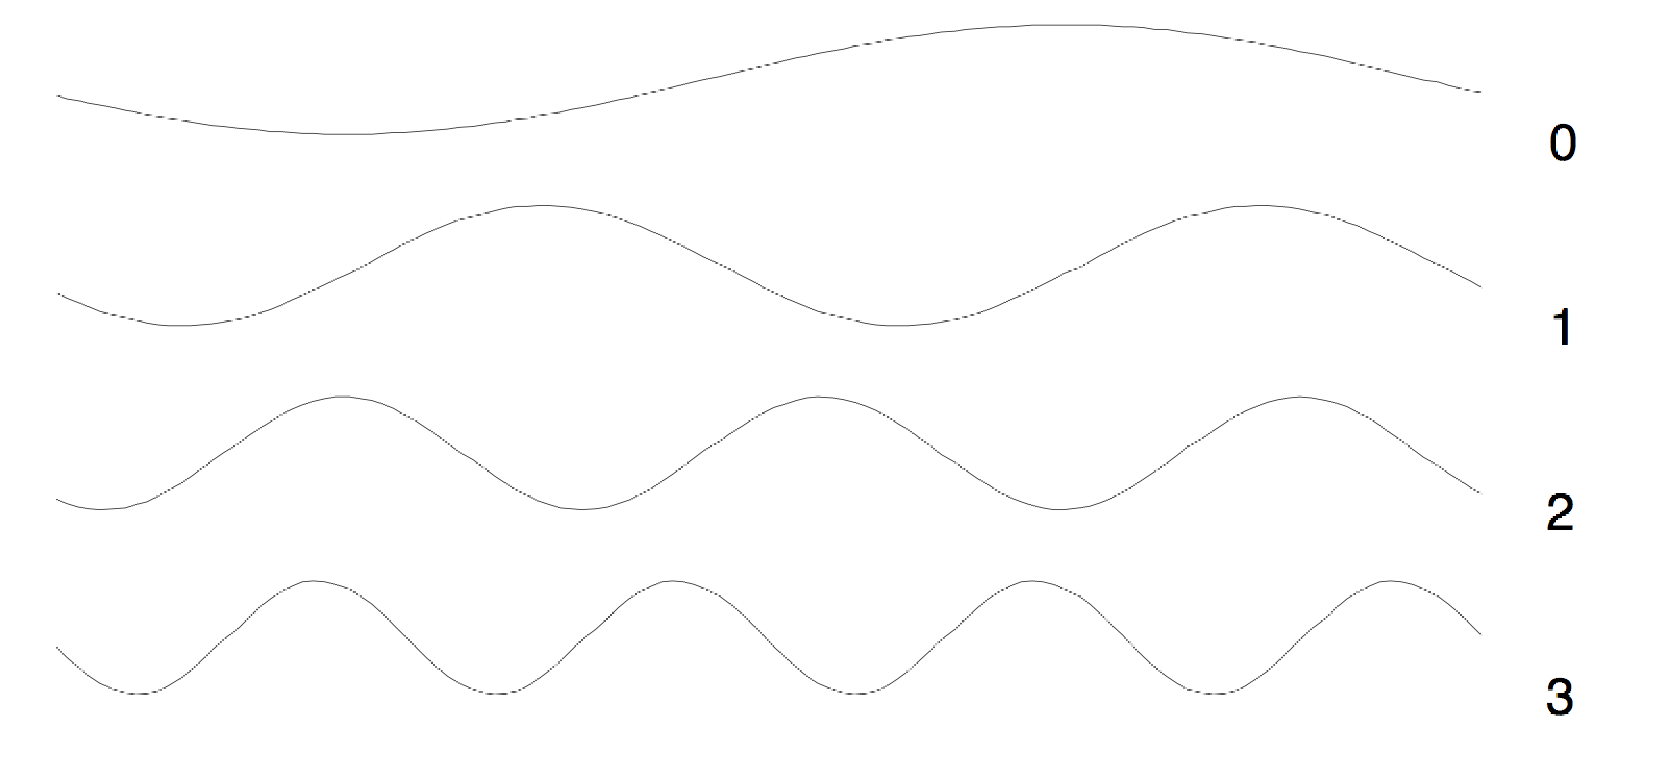
\includegraphics[width=0.45\textwidth]{Fig/chapter2/DFT.eps}
%	}
%	\caption{离散傅里叶压缩数据\cite{KeoghDimReduction}}
%	\label{fig-chapter2-DFT}
%\end{figure}

\textbf{离散傅里叶变换:}
离散傅里叶变换(Discrete Fourier Transform, DFT)\cite{DFT}是时间序列数据降维的常用方法,并且已有许多扩展和改进方案被提出\cite{fastDFT,rafiei1997similarity,rafiei1999on}。
其基本思想是任何一个信号,不管其多复杂,都可以分解为有限个正弦和余弦曲线的叠加。每条曲线可以由一称为傅里叶系数的复数表示\cite{Shatkay1995The}。此时,我们时间序列由时域变换到频域了。使用频域的好处有很多,其最重要的就是能进行数据压缩。一条长度为$n$的信号(即时间序列)可以被分解为$n$个正/余弦曲线,且这$n$个曲线能重新组合成原来的信号序列。但由于$n$个曲线中存在着许多振幅较低的,这些低振幅曲线对重新构建原来的信号的贡献较低。因此,其对应的低振幅系数可以被丢弃掉,而保留那些振幅较高的系数。这些保留的系数重新组合所构成的信号数据与原始信号数据相比,并没有太多的信息丢失。因而,达到了使用少量数据来表示原始信息的目的。
此外,文献\cite{Shatkay1995The}中提出了帕斯瓦尔定理(Parseval's law),即
原始时域内信号数据间的欧氏距离等于变换后频域内系数间的欧氏距离。因此,若经离散傅里叶变换且将低振幅的系数丢掉后,使用剩下的系数计算距离,所得到的结果必然是原始欧氏距离的下界(丢失的数据都是正数)。文献 \cite{KeoghDimReduction}提出了基于该下界的剪枝方法。

%为将以长度为$n$的时间序列降低到$N$维特征。我们调用离散傅里叶变换并保留了$N/2$个系数。保留$N/2$而不是$N$的原因是每个系数是一个复数,我们需要同时保留实部和虚部的值。图\ref{fig-chapter2-DFT}介绍了使用离散傅里叶变换进行压缩数据的思想。首先对左图原始信号$X$进行傅里叶变换。然后只保留了如右图振幅较高的4个曲线。接着,我们利用保留的4个系数恢复出原始轨迹的近似轨迹$X'$。在我们的分布式查询中,可以通过发送压缩后的 系数数据以达到降低通信开销的目的。

\textbf{小波变换:}
小波变换(Wavelet Transform) 将信号分解为一系列基/母小波函数的和与差的组合,这一点与离散傅里叶变换类似。但它们之间也有许多的不同点。其中一个重要的区别是,小波在时间上是局部的,即小波系数只代表原始数据中的一小部分子段。这也是“小波”这一名词的由来,“小波”就是小区域、长度有限、均值为0的波形。
而傅 里叶系数总是代表着数据的全局信息。对于一些需要研究数据局部信息的应用来说,具有多解析度特性的小波变换更为适用。
%
%\begin{figure} [t]
%	\centering
%	\subfigure[压缩前后数据]{
%		\label{fig:haar}
%		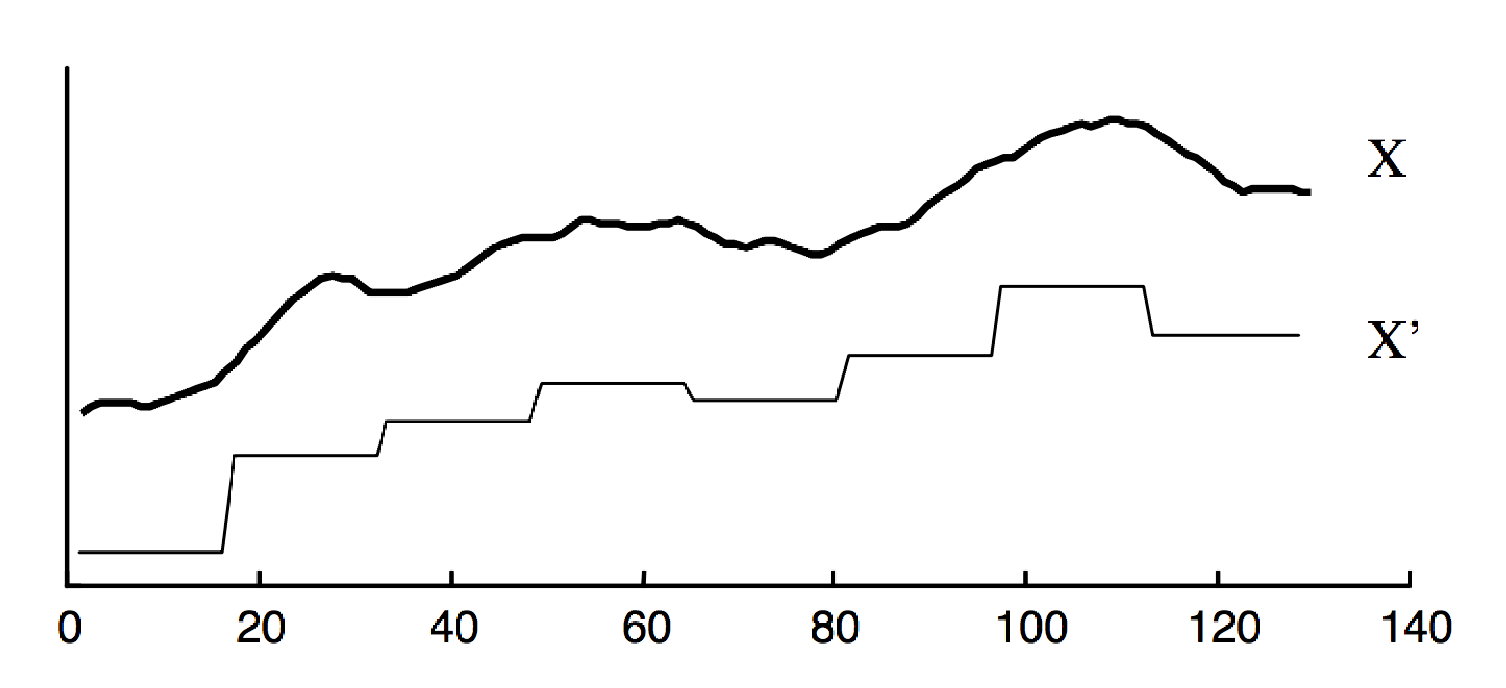
\includegraphics[width=0.45\textwidth]{Fig/chapter2/Haar.eps}		
%	}
%	\subfigure[小波系数]{
%		\label{fig:haarcoeff}
%		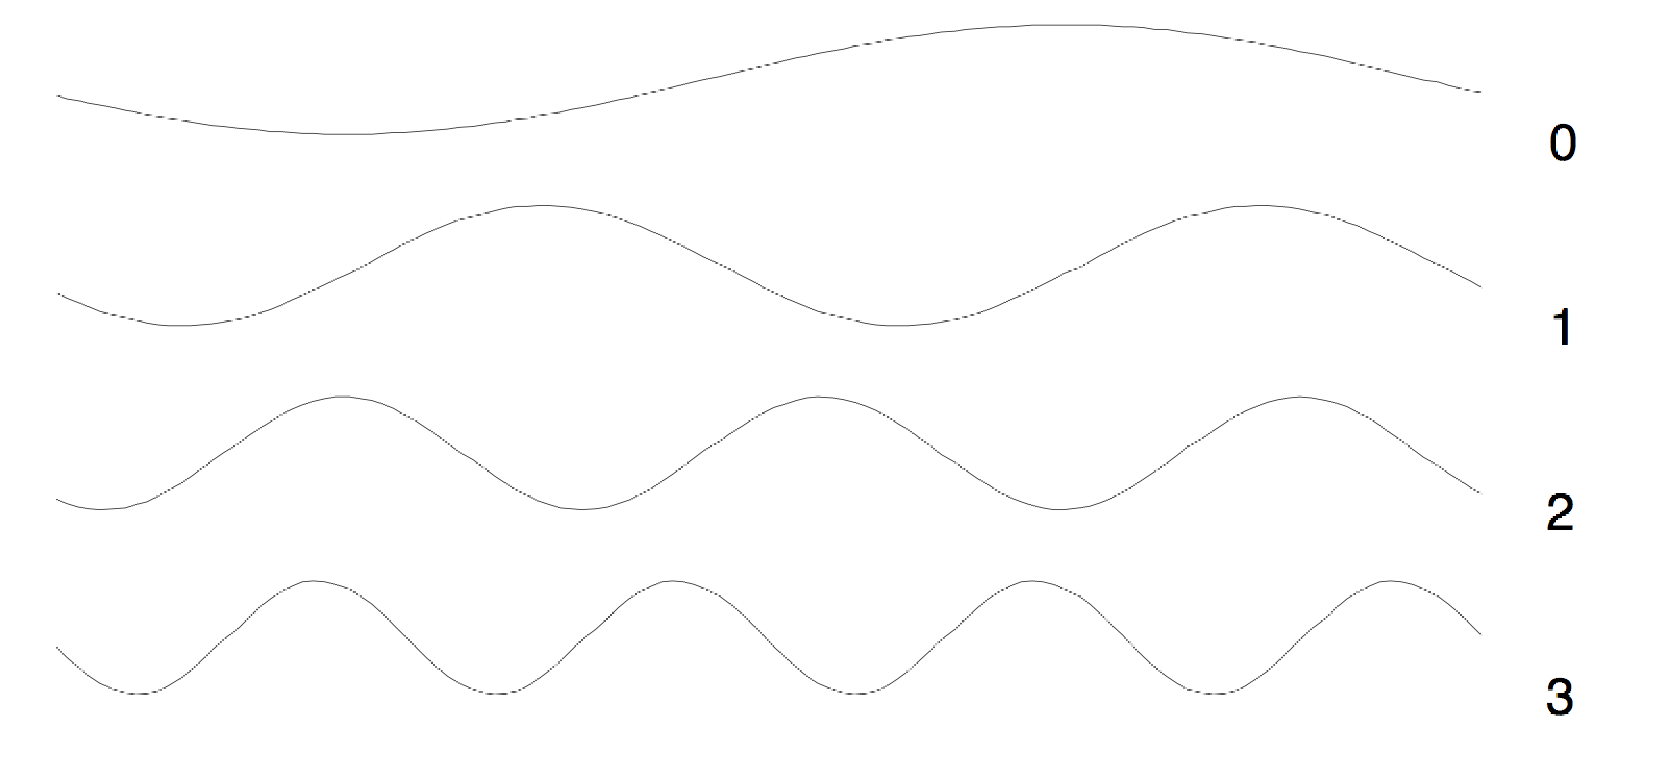
\includegraphics[width=0.45\textwidth]{Fig/chapter2/DFT.eps}
%	}
%	\caption{哈尔小波压缩数据\cite{KeoghDimReduction}}
%	\label{fig-chapter2-haar}
%\end{figure}
当原始信号/时间序列数据被小波分解之后,会得到一个小波系数序列。该序列的前几个系数包含了数据的总体信息,是对原始信号数据的粗粒度估计。
而其余的系数则包含着数据局部的细节信息。因此使用 小波变换压缩数据,就是通过只保留前几个系数,以大体上逼近 原始的数据,达到降维的目的。其代价是损失一些局部的细节信息。这一点跟傅里叶变换进行压缩一样,两者都是有损压缩。近年来,小波变换由于其同时保持了时域和频域的特征(傅里叶只包含了频域特性),在数据压缩、过滤、分析等领域得到广泛应用。

%哈尔小波是表达和计算都最简单的一种小波。它的基函数是均值和差值函数。
%Chan等人证明了原始时域内信号数据间的欧氏距离等于变换后哈尔小波系数间的欧氏距离\cite{chan2003haar}。
%图\ref{fig-chapter2-haar}展示了经过哈尔小波变换压缩数据的过程。对于给定的时间序列$X$,经过哈尔小波变换后,我们只保留了右图所示前8个系数。利用这8个系数,我们可以计算出原始时间序列的近似值$X'$。在我们的分布式查询中,可以通过发送这些前面的哈尔小波系数以达到降低通信开销的目的。

\textbf{奇异值分解:}
尽管奇异值分解(Singular Value Decomposition, SVD)方法已经成功应用于图像和多媒体数据的分析中。最近的工作表面,其也可以被应用于时间序列数据的索引和压缩中。相比于前面介绍的几种方法都是对单一轨迹进行压缩,各个轨迹之间相互独立。奇异值分解不是针对单个时间序列对象进行压缩,而是对全局数据进行整体变换,以得到整体数据的压缩结果。
%其分解过程如下,首先将整个数据集进行变换,在原始的数据空间中顺序地找一组相互正交的坐标轴,其中沿第一个坐标轴方向的方差最大,而在与第一个坐标 轴正交的平面上,沿第二个坐标轴方向的方差最大,在于第一个坐标轴以及第 二个坐标轴正交的平面中,沿第三个坐标轴的方向方差最大,依次类推。对于长度为$n$的时间序列,可以通过奇异值分解找到$n$个满足条件的坐标轴。为了达到降维的目的,
%取前$N$个坐标轴构成一个$N$维的空间来近似原来的$n$维空间,这样就将一个$n$维空间变换成了$N$维的近似空间,且使用上述方法选择 的$N$个坐标轴所张成的空间中,数据的损失最小。

\subsection{传统在线时间序列压缩算法}
离线的轨迹压缩算法可以充分根据轨迹的所有信息来获取较好的压缩效果。但对于实时在线场景,我们无法事先得到完整的轨迹数据,因而需要在线算法来进行实时压缩。相比于离线压缩算法,降低计算开销是在线算法的重要内容,它需要快速确定是否要保留刚刚到来的轨迹点。为此,我们将介绍几种典型的在线算法。

\textbf{蓄水池算法:}
蓄水池算法(Reservior Sampling Algorithm)\cite{Reservoir}的思想是为每个时间序列维持一个大小为$R$的缓冲区,并用这$R$个点来近似原始轨迹。由于轨迹数据是持续增加的,无法知道轨迹的最终长度。因而,该算法所要解决的核心问题就是无放回替换,即当一个点从缓冲区删除掉后,不能再将它取回。它的做法是,首先将前$R$个轨迹点放入缓冲区,当新的轨迹点到来时,判断该点是否需要放入缓冲区。具体地,当第$k$个点到来时($k>R$),该算法以$R/k$的概率判断该点是否需要加入缓冲区。如果判断结果正确,则从现有的轨迹点中随机删除一个点,并将新点加入。该算法的时间复杂度为$O(R\cdot(1+\log N/R))$,因此效率较高。但它没有考虑轨迹的时间或空间属性,因而近似轨迹无法保留轨迹的原始特征。

\textbf{滑动窗口算法:}
与蓄水池算法不同的是,滑动窗口算法\cite{ICDMSiding,EDBTSliding}的思想是维护一个不断增大的缓冲区,并用缓冲区中的轨迹来近似原始轨迹。它的算法过程是,首先选取第一个点作为锚点,用$\vp_a$来标识,然后将下一个点加入滑动窗口中。当新点$vp_{i}$加入后使用$\overline{\vp_a \vp_i}$来拟合窗口中所有点组成的字轨迹。若$\overline{\vp_a \vp_i}$拟合误差小于给定的阈值,则继续加入新点。否则,将$\vp_a$与$\vp_{i-1}$之间的点从缓冲区删除,并使用$\vp_{i-1}$作为新的锚点。该算法能有效保留轨迹的原始时空特征。

%\begin{figure}
%	\centering
%	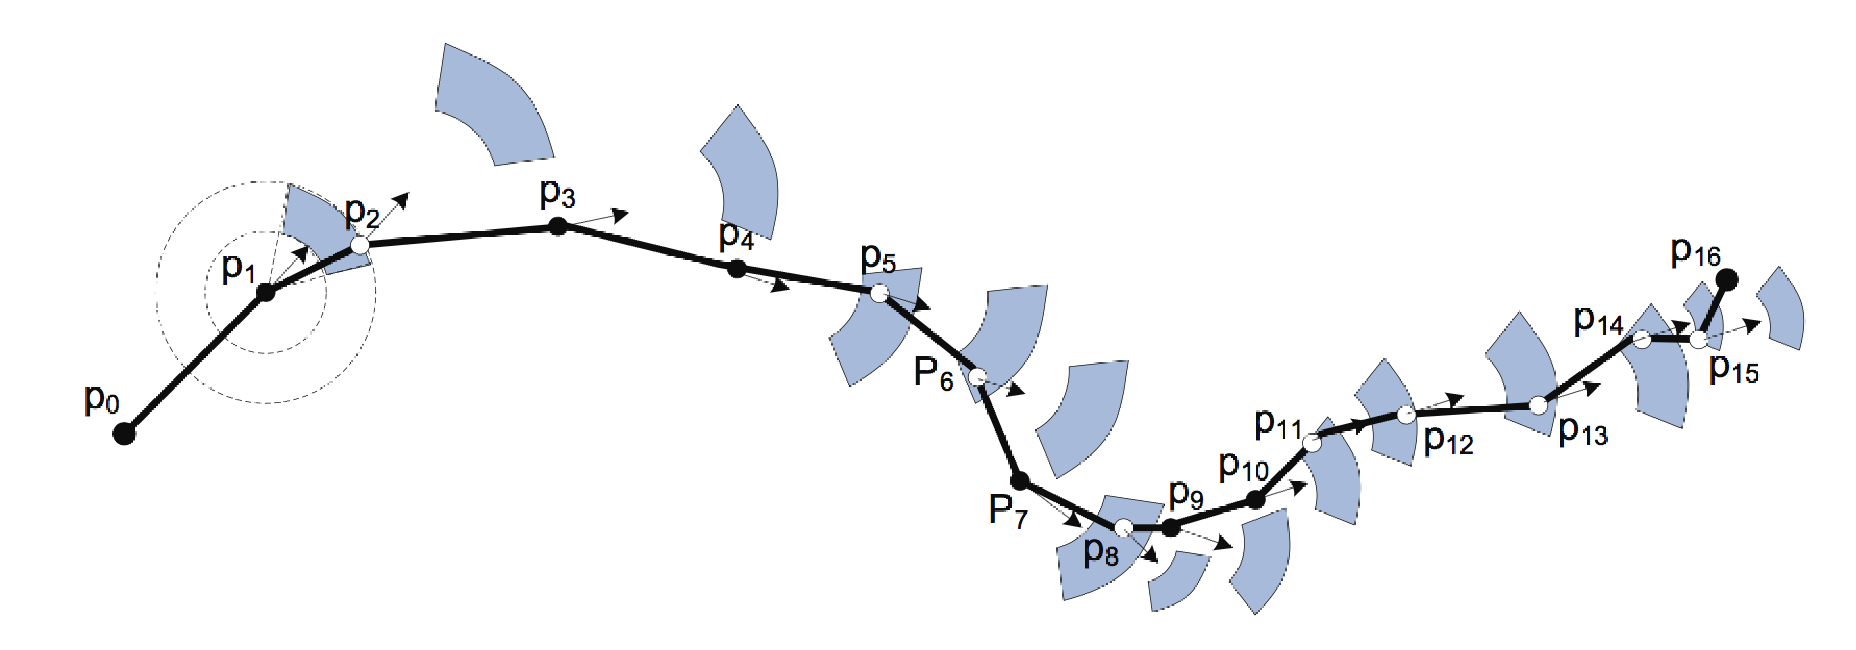
\includegraphics[width=0.73\textwidth]{Fig/chapter2/safearea}
%	\caption{基于安全区的压缩算法\cite{Zheng2011Computing}}
%	\label{fig-chapter2-safeare}
%\end{figure}

\textbf{基于安全区的算法:}
以上两个压缩算法没有考虑轨迹中所蕴含的速度和方向等特征,为此Potamias\cite{SSDBMSample}等认为,一个轨迹点只要能表示轨迹发生了改变,就应该包含到最终的压缩轨迹中。而如果一个点可以从之前的运动中通过插值或位置预测等方法计算出来,那么就可以将其舍弃。因此,他们认为在轨迹压缩过程中应该考虑速度和方向这些特征,因为这些可以用来预测轨迹的位置。
因而中提出了一种阈值导向的采样算法,即基于安全区的算法,来减少轨迹中的冗余数据点。
该算法基本思路是使用最后两个轨迹点以及速度及方向预设的阈值来计算一个安全区域,以此判断一个新采集到的轨迹点是否含有重要的信息。如果该点位于安全区域之内,则认为它是多余的,可以被舍弃; 如果该点位于安全区域之外,则将其保留在压缩轨迹中,因为此时运动方向或 者速度己经发生了改变。
%图\ref{fig-chapter2-safeare}举例介绍了本算法。假设$\vp_0$和$\vp_1$包含在压缩轨迹中,由于各轨迹点本身包含了角度和速度信息。当采集到轨迹点$\vp_2$时,根据物体在$\vp_1$ 处的运动速度、运动方向、速度和方向的误差阂值,以及$\vp_1$与$\vp_2$之间的时间 间隔,可以构建出一个扇形区域,即物体在采集到$\vp_2$点的可能位 置。图中$\vp_2$在该扇形区域之内,因此它并没有蕴含太多信息,可以将其舍 弃。接着,当采集到轨迹点$\vp_3$时,又可以构造出该时刻的安全区域。由于 $\vp_3$不在这个安全区域之内,因将它保留。依次类推,最终保留的压缩轨迹为$\{\vp_0,\vp_1,\vp_3,\vp_4,\vp_7,\vp_9,\vp_{10},\vp_{16}\}$。

\subsection{基于路网结构的轨迹压缩算法}
上述传统时间序列算法受限于基于欧氏空间,而人、车辆等运动轨迹往往受限于路网结构。简单使用欧氏距离的度量方式,无法有效刻画这些对象的移动行为。随着城市路网结构数据的完善,结合路网数据的轨迹压缩方法不断被提出\cite{YinW04,nonmaterialized,DMDL2,MDL1}。这些算法往往需要将轨迹数据进行地图匹配预处理,以将原始轨迹点映射到路网中。这样做的好处有:(1).轨迹点落在路网结构上更能直观表达位置信息。(2).连续变动的多个轨迹点可能对应同一个路段,因而使用路段表达能有效的降低数据存储开销。此外,一个城市中的路网线段是有限的,而采集的轨迹点时无限的。使用路网数据表达原始位置,能有效降低数据表示的复杂度。

\textbf{Non-materialized算法}文献\cite{YinW04}提出了Non-materialized算法来压缩数据,他首先将原始轨迹变成路网序列数据,接着将上述结果转换成路口 的序列数据,从而压缩轨迹。文献\cite{nonmaterialized}提出了基于最短路径和链接相结合的压缩算法。所谓最短路径就是,如果一条移动轨迹与其起始和终点的最短路径相一致,那么可以用头尾两条路段来表示整条轨迹。链接的思想上,假设司机在两个路段间的行驶轨迹都是沿着最小转角的路段行驶,并将相邻两路段的头尾连接起来拼凑成更长的轨迹。

\textbf{基于MDL模型的算法}文献\cite{DMDL2,MDL1}把轨迹压缩问题转换成一个最优化的问题,其目标是寻找一条近似轨迹,使得压缩率尽可能高,且该轨迹与原始轨迹相似度尽可能高。文章引入信息论中的最小描述长度模型 (Minimal Description Length,MDL),来 表示最 优 化 压 缩 率 和 相 似 度 组 成 的 目 标 函 数。
MDL 模 型 是 信 息 论 中 的 常 用 模 型 ,有 两 个 部 分 组 成 ,分 别 是$L (H )$ 和 $L (D|H )$。$L (H )$ 为假 设 条 件 ;$L (D|H )$为在 此 假 设 条 件 下 ,数 据 的 描 述 情 况 。在对应到轨迹 数 据 压 缩 中 ,$L (H )$ 表 示 压 缩 后 的 轨 迹;$L (D|H )$表示近似轨迹与原始轨迹之间的误差。根据 MDL原则,只要找到一条路径,使得
 $L(H)+L (D|H )$最 小 ,那 么 这 条 路 径 就 是 满 足 目 标 的 路 径 。
% 这两部分的定义如下:
% \begin{eqnarray}\label{eq:MDL}
% MDL(D,H)&=&L(H)+L(D|H) \\
% L(H)=\log_{2}(\delta *\frac{|T_{MMTC}|}{T'}) &;&\quad L(D|H)=\log_{2}(\delta *D_{total}(T_{MMTC},T'))
% \end{eqnarray}
% 其 中,$|T_{MMTC}|$  代表压缩后的轨迹的长度,$|T′|$是 原始轨迹经地图匹配后的轨迹,$D_{total}(T_{MMTC},T')$是指$T_{MMTC}$  和 $T′$之 间 的 距 离。
% 整个算法过程如下:从  $T′$的 起 点$\vp_{1}$开 始 ,把 后 面 的 点 都 遍 历 一 遍 ,找 到$\vp_{1}$ 与$\vp_{i}$之间的最短路径$SP_{1i}$,计算$T′_{1i}$和$SP_{1i}$之间的$MDL_{1i}$,找出使$MDL_{1i}$最小的$i$ 值。用$SP_{1i}$来近似替代$T′_{1i}$。然后从$\vp_{i}$开始,重复上述步骤,直到轨迹的终点。把所有找到的$SP_{ij}$ 连在一 起 便 是 最 终 的 $T_{MMTC}$。
 该算法在高频率的采样数据集和稀疏的路网结构下有较好的效果。此外针对估计分布不均的情况,\cite{hufmmanCompres}利用哈夫曼思想编码思想的轨迹压缩方法,即出现频率越高的轨迹段编码越长。
 
 \subsection{语义压缩算法}
 原始轨迹和路网轨迹尽管能很好地记录移动物体的运动踪迹,但是对于人们理解轨迹的含义却帮助不大。因为人们阅读轨迹时,无法直观了解经纬度坐标代表的意义。因此出现了利用 POI、标 志 物 、路 口 和 路 段 来 表 示 车 辆 的 行 驶 过 程 ,人 们 阅 读 语 义轨迹时,能明确知道轨迹的起点、终点以及行驶经过的路段。

\textbf{基于事件的压缩算法}文献\cite{Sementick,RichterSL12} 提 出 了 仅保 存 有 意 义 的 状 态 和 事 件的语 义 轨 迹 压 缩。它把 一 条 轨 迹 拆 分 为 若干连续的事件。事件包括行驶的路段,如从边$a$直走到达边$b$,以及方向的改变,如在$b$路口左转到达边 $c$。这种描述方法,会用一条边来表示若干个点,以而达到压缩的目的。

%该方法压缩后的轨迹数据便于阅读和理解,但方法本身也存在着压缩和解压时间长、位置信息丢失等问题。这导致其应用场景有限。

\textbf{基于摘要的压缩算法}文献\cite{STMaker} 针对现有语义压缩方法未考虑速度、方向等问题,提出了利用 轨 迹 摘 要 数据的压缩 框 架。在文章中,他们考虑了道路等级、路宽、速度、停车次数和U形转弯次数这六个特征表示摘要数据。其框架包含``划分''和``汇总''两个阶段。在划分阶段,根据之前提取的6个特征,把轨迹切分为几段 子轨迹 以使得每段子轨迹内部具有相似的特征,同时子轨迹之间的特征差异较大。在每段 内,选取最具代表性的特征来描述这段的移动过程。
在 汇总 阶 段 ,使用每段的 特 征来描述轨迹形式过程。该通过提取轨迹概要数据,不仅压缩了数据量,而且也便于人们 理 解 轨 迹 的 行 为 。
文 献 \cite{Makesense}介绍了该算法的演示系统 ,要 求 输 入 一 条 原 始 轨 迹 序 列 , 并输出一段文字,用以描述轨迹的行驶特征以及经过的重要位置。

综上所述,语义压缩后得到的轨迹,便于阅读理解且显著地减少了空间开销。但缺点是丢 失了具体的经纬度信息,从而不能支持具体的点查询。

%\section{轨迹索引}\label{sec-c2-index}


\section{轨迹距离度量}\label{sec-c2-measures}
轨迹距离的定义是轨迹挖掘中的核心内容之一。其度量方式可以分为3大类:传统时间序列距离、针对轨迹时空特性专门设计的距离(简称为时空轨迹距离)、以及针对轨迹语义属性设计的距离(简称为语义轨迹距离)。下面我们将介绍每一类的经典度量方式及其特点。

\subsection{传统时间序列距离}
传统时间序列距离广泛应用于时间序列数据分析上如:语音识别、股票期货等价格分析。其典型距离有$L_{p}$距离、动态时间弯曲距离和最长公共子串距离。

\textbf{$L_{p}$及欧氏距离:}
$L_{p}$(闵可夫斯基距离)距离是$L_1$(曼哈顿距离)、$L_2$(欧氏距离)以及$L_\infty$(切比雪夫距离)等多个距离的总称。使用这一类距离的前提是,任意两条轨迹具有相同的长度。
在该类距离中欧氏距离是最常用的一个,其计算方式是对应轨迹点间欧氏距离的累加和。特别的,给定两条轨迹分别为${\cal{Q}}=\{\vq_{1},\vq_{2},\cdots,\vq_{n}\}$和${\cal{P}}=\{\vp_1,\vp_{2},\cdots,\vp_{n}\}$,其对应的任意一对点$\vq_{i}$和$\vp_{i}$间的欧氏距离定义如公式\ref{eq:edpoint}所示。在此基础上,公式\ref{eq:edtrajecotry}定义了两条轨迹间的欧氏距离。轨迹间欧氏距离是对应点欧氏距离的累加和。拓展到$L_{p}$距离,其距离为对应点的$p$范数距离的累加。以欧氏距离为代表的$L_{p}$距离具有计算简单的优点。但也存在着查询结果易受噪声数据影响的缺点。
\begin{eqnarray}
ED(\vq_{i},\vp_{i})&=&||\vq_{i} - \vq_{i}|| \\ \label{eq:edpoint}
ED({\cal{Q}}, {\cal{P}})&=&\sum\nolimits_{i=1}^{n}ED(\vq_{i},\vp_{i}) \label{eq:edtrajecotry}
\end{eqnarray}
%\begin{eqnarray}\label{eq:edtrajecotry}
%ED({\cal{Q}}, {\cal{P}})=\sum_{i=1}^{n}ED(\vq_{i},\vp_{i})
%\end{eqnarray}


\textbf{动态时间弯曲距离:}
相比于欧氏距离,动态时间弯曲距离能处理两条轨迹长度不同的情况。
假设给定两条轨迹分别为${\cal{Q}}=\{\vq_{1},\vq_{2},\cdots,\vq_{n}\}$和${\cal{P}}=\{\vp_1,\vp_{2},\cdots,\vp_{m}\}$
它们之间的动态时间弯曲距离可由定义\ref{eq:ch2-dtw}中的方式递归计算。其中${\cal{Q}}_{1,n-1}$代表轨迹$\cal Q$从第$1$到第$n-1$个点构成的子轨迹。由于动态时间弯曲距离不满足三角不等式,因此它不是一个度量准则。
其尝试将将两条轨迹的点以最小的距离和对应起来。
\begin{equation}\label{eq:ch2-dtw}
DTW({\cal{Q}}_{1,n}, {\cal{P}}_{1,m})=||\vq_{n}-\vp_{m}||+min \begin{cases}
DTW({\cal{Q}}_{1,n-1}, {\cal{P}}_{1,m-1})  \\
DTW({\cal{Q}}_{1,n-1}, {\cal{P}}_{1,m})  \\
DTW({\cal{Q}}_{1,n}, {\cal{P}}_{1,m-1})
\end{cases}
\end{equation}


\textbf{最长公共子串距离:}
最长公共子串距离也不要求两条轨迹具有相同的长度。其定义如公式\ref{eq:ch2-lcss}所示。与前两个距离相比,最长公共子串距离对于数据含噪声的情况处理结果更加鲁棒。但它需要额外参数$\epsilon$来约束两个点空间的相似性。
最近提出的EDR和EDP距离同样也是设计出来处理带噪声的数据,其处理噪声的效果比最长公共子串距离还好。但由于所使用的广泛性不高,故不作详细介绍。
\begin{eqnarray}\label{eq:ch2-lcss}
LCSS({\cal{Q}}_{1,n}, {\cal{P}}_{1,m})= \begin{cases}
0 & if \, n=0 \lor m=0  \\
1+ LCSS({\cal{Q}}_{1,n-1}, {\cal{P}}_{1,m-1}) & if \,  ||\vq_{n}-\vp_{m}||<\epsilon  \\
\max \{LCSS({\cal{Q}}_{1,n-1}, {\cal{P}}_{1,m}) ,\\LCSS({\cal{Q}}_{1,n}, {\cal{P}}_{1,m-1})\} & otherwise
\end{cases}
\end{eqnarray}



\subsection{时空轨迹距离}
相比传统时间序列数据,轨迹数据独有空间属性。为刻画空间属性的影响,许多工作提出了新的距离。其中典型的有基于最小包围盒的距离、豪斯多夫距离和弗雷歇距离。

\textbf{基于最小包围盒距离 :}
基于最小包围盒距离利用给定轨迹线段间的最小包围盒来快速计算轨迹线段间的距离。假设$B_{1}$和$B_{2}$分别代表轨迹线段$L_{1}$和$L_{2}$间的最小包围盒。$D_{min}(B_{1},B_{2})$距离代表$B_{1}$内任意一轨迹线段与$B_{2}$内任一轨迹线段间距离的下界。其计算方式如公式\ref{eq:ch2-MBR}所示。
\begin{eqnarray}\label{eq:ch2-MBR}
D_{min}(B_{1},B_{2})=\sqrt{(\Delta(B_{1}.[x_{l}, x_{u}], B_{2}.[x_{l},x_{u}])  )^2+(\Delta(B_{1}.[y_{l}, y_{u}], B_{2}.[y_{l},y_{u}]) )^2 }
\end{eqnarray}
其中两个区间的距离定义如下:
\begin{equation}\label{eq:ch2-DisInternal}
\Delta([l_{1}, u_{1}], [l_{2},u_{2}]) =\begin{cases}
0 & if \, [l_{1}, u_{1}] \cap [l_{2},u_{2}] \neq 0   \\
l_{2}-u_{1} & if \, u_{1} < l_{2}   \\
l_{1}-u_{2} & if \, u_2 < u_{1}
\end{cases}
\end{equation}


\begin{figure}[t]
	\begin{minipage}[t]{0.5\linewidth}
		\centering
		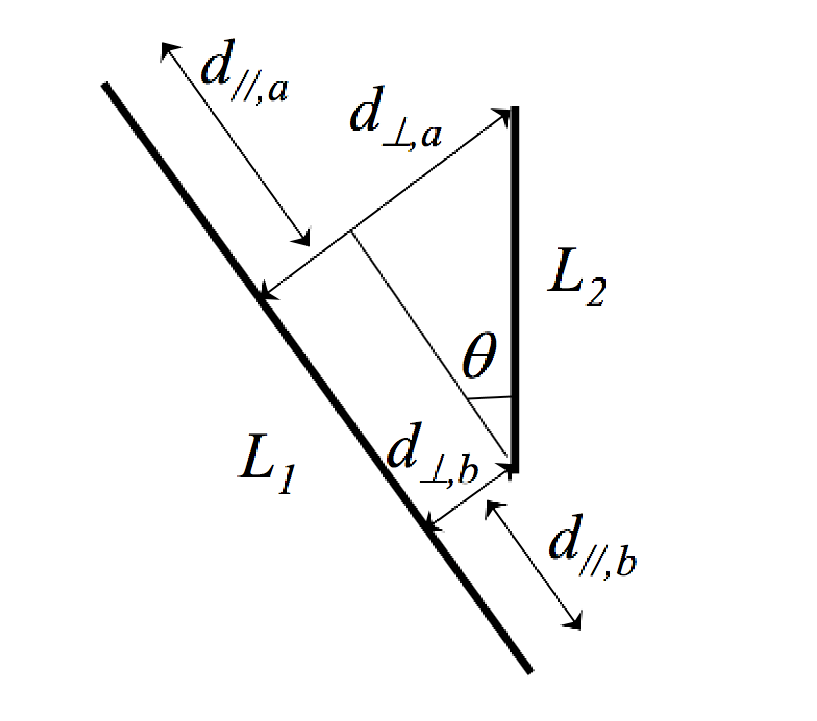
\includegraphics[width=2.5in]{Fig/chapter2/Hausdorff}
		\caption{豪斯多夫距离}
		\label{fig-chapter2-Hausdorff}
	\end{minipage}%
	\hfill
	\begin{minipage}[t]{0.5\linewidth}
		\centering
		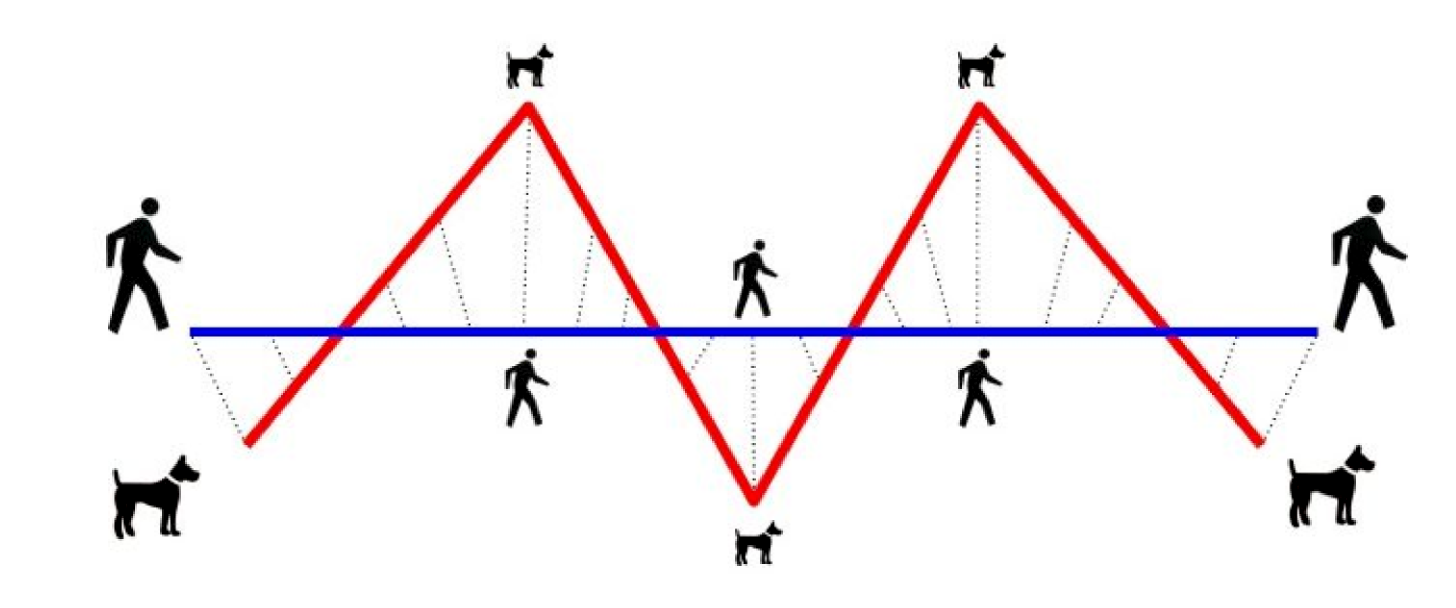
\includegraphics[width=3in]{Fig/chapter2/dogpeople}
		\caption{弗雷歇距离}
		\label{fig-chapter2-Frechet}
	\end{minipage}
\end{figure}

\textbf{豪斯多夫距离:}
豪斯多夫距离是用来衡量两个轨迹段的相似度。给定轨迹段$L_{1}$和$L_{2}$,豪斯多夫距离定义如公式\ref{eq:ch2-hausdorff}所示,表示为3个带权重距离的累加和。其中$d_{\perp}$表示两个轨迹段的垂直距离,$d_{||}$代表轨迹段间的平行距离,$d_{\theta}$代表轨迹段间的夹角距离。这些几何意义如图\ref{fig-chapter2-Hausdorff}所示。
而$w_{\perp}$、$w_{||}$和$w_{\theta}$为上述三个距离在距离的权重,这些权重值可以随着应用场景的不同而调整相应的值。
\begin{eqnarray}\label{eq:ch2-hausdorff}
Hausdorff(L_{1},L_{2})=w_{\perp} \cdot d_{\perp} + w_{||}\cdot d_{||} +w_{\theta} \cdot d_{\theta} \nonumber \\
d_{\perp} =\frac{d_{\perp,a}^2 + d_{\perp,b} ^2}{d_{\perp,a} +d_{\perp,b}}, \qquad d_{||}=\min\{d_{||,a}, d_{||,b}\},\qquad d_{\theta}=||L_{2}||*\sin{\theta}
\end{eqnarray}
在上述公式中$d_{\perp,a}$和$d_{\perp,b}$分别表示$L_{1}$和$L_{2}$间的垂直距离,$d_{||,a}$和$d_{||,b}$分别表示$L_{1}$和$L_{2}$间的平行距离,$\theta$代表两线段间的夹角。

%\begin{figure}
%	\centering
%	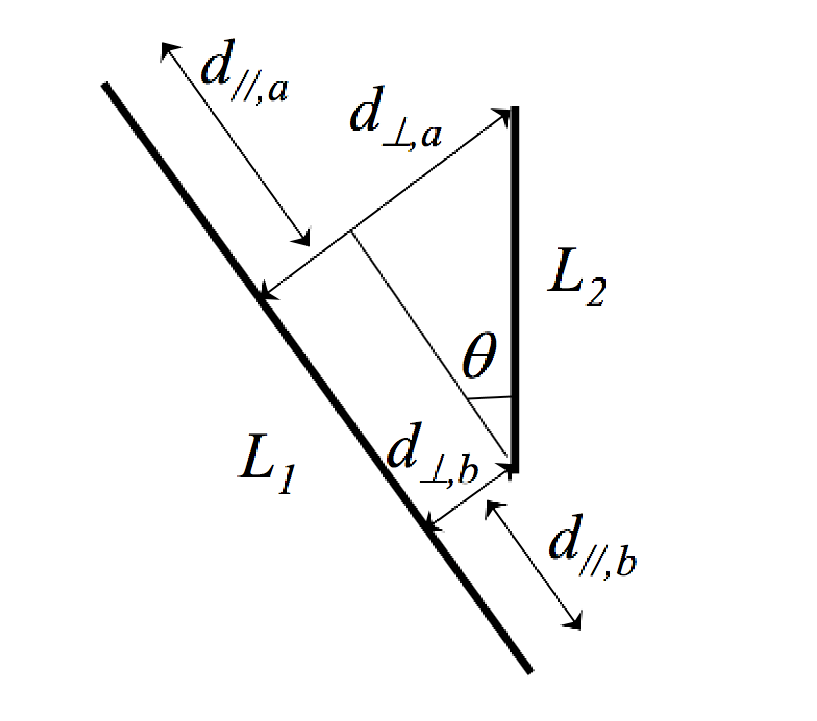
\includegraphics[width=0.43\textwidth]{Fig/chapter2/Hausdorff}
%	\caption{豪斯多夫距离}
%	\label{fig-chapter2-Hausdorff}
%\end{figure}

\textbf{弗雷歇距离:}
弗雷歇距离通俗的讲就是狗绳距离。如图\ref{fig-chapter2-Frechet}所示人和狗的轨迹, 两者之间有一条狗绳约束。主人走路径A,狗走路径B,各自走完这两条路径过程中所需要的最短狗绳长度就是弗雷歇距离。
%\begin{figure}
%	\centering
%	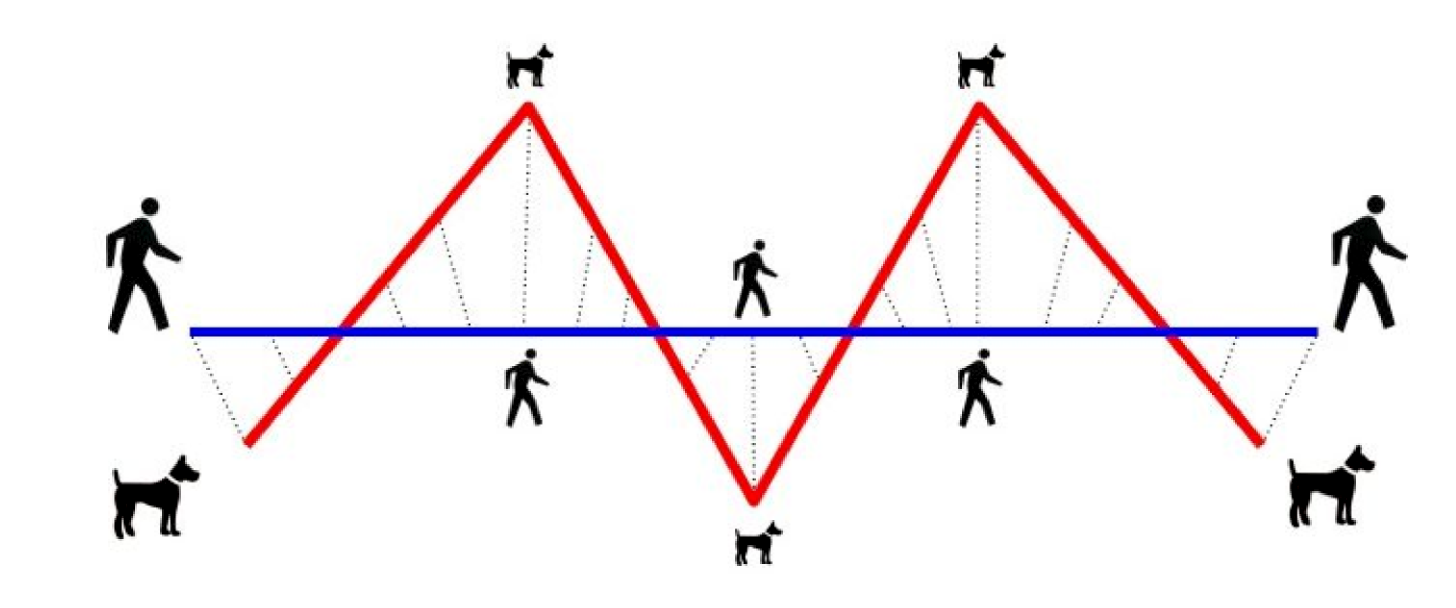
\includegraphics[width=0.73\textwidth]{Fig/chapter2/dogpeople}
%	\caption{弗雷歇距离}
%	\label{fig-chapter2-Frechet}
%\end{figure}

\subsection{语义轨迹距离}
语义轨迹的特点是将原始轨迹中的坐标映射到一个语义信息上,如给点标注为“学校”。从而使得原始的坐标序列变为语义信息的序列。现有语义轨迹度量方式的思想就是从语义和空间两个角度来考虑相似性,但它们的实现方式各不相同。

%\begin{figure}
%	\centering
%	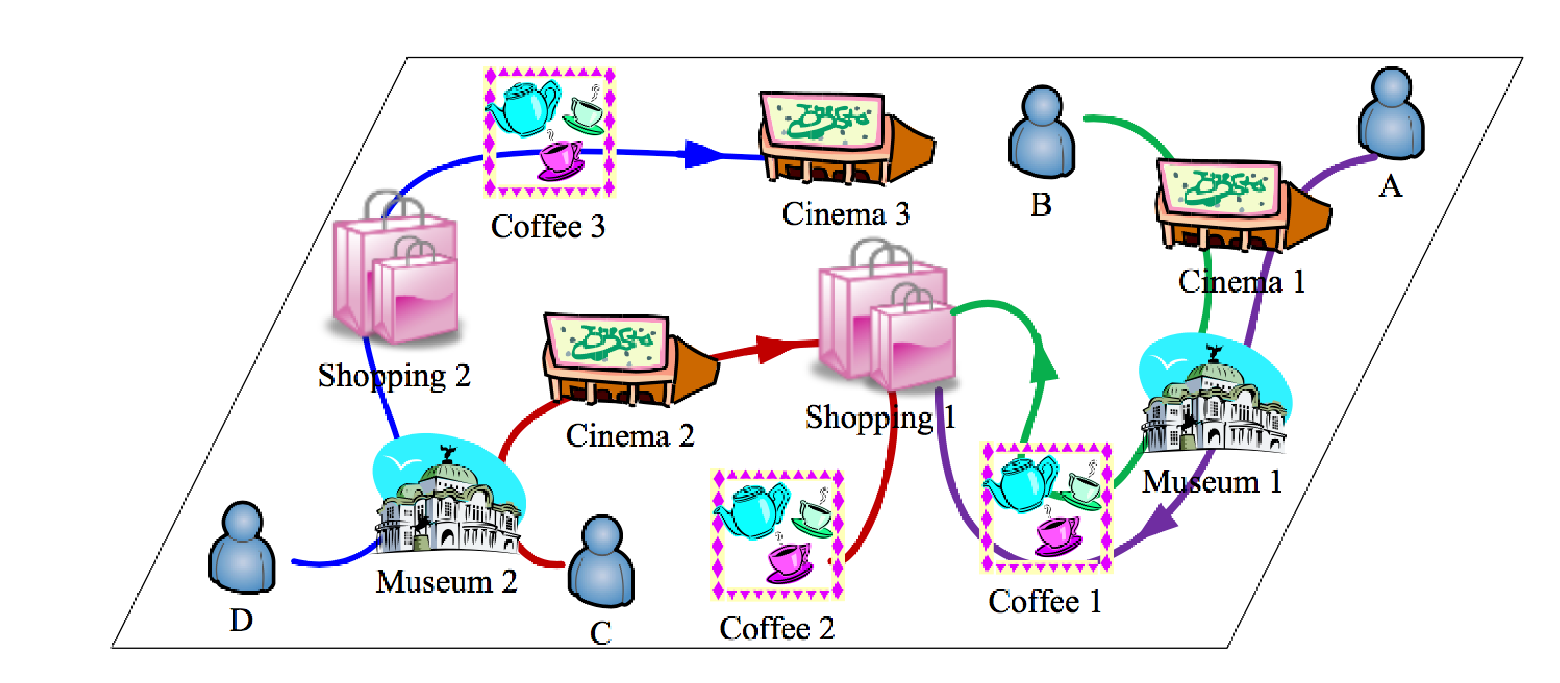
\includegraphics[width=0.73\textwidth]{Fig/chapter2/catagorySementic}
%	\caption{基于分类属性的语义轨迹\cite{Xiao}}
%	\label{fig-chapter2-category}
%\end{figure}
文献\cite{Xiao}提出了基于位置分类属性的语义轨迹分析方法。该方法首先将POI分成博物馆、医院、学校等若干个类别,然后给原始轨迹的每个点赋予类别属性。最后使用类别属性的序列进行相似度计算。
文献\cite{Liu012}利用轨迹空间距离和语义距离的比值来作为最终两个轨迹的相似度。其计算方式如公式\ref{eq:ch2-Liu012}所示,其中$geoDist$代表了两条轨迹的空间距离,$semRatio$代表了两条轨迹间的语义距离。其空间距离考虑了轨迹中心点间的距离、轨迹长度的差别和轨迹间的角度。其语义距离使用最长公共子串距离除以短轨迹长度来表示。$\alpha$用于调节着空间和语义距离的比重。
\begin{eqnarray}\label{eq:ch2-Liu012}
totalDist(t_{1},t_{2}) =geoDist(t_{1},t_{2})\cdot \frac{1}{1+\alpha \cdot semRatio(t_{1},t_{2})}
\end{eqnarray}

文献\cite{Kaiser,ShangDYXZK12,ZhengYZXSZ15}给空间距离和语义距离以不同权重,并用它们的权重和作为轨迹或轨迹点的相似度。其定义形式如公式\ref{eq:ch2-add}所示。其中文献\cite{Kaiser}中要求被查询轨迹要完全包含待查询轨迹的所有语义信息。文献\cite{ShangDYXZK12}不是给每个点一个标签属性,而是给每条轨迹一个标签信息。文献\cite{ZhengYZXSZ15}提出了快速求解近似查询结果的方法。
\begin{eqnarray}\label{eq:ch2-add}
totalDist(t_{1},t_{2}) = \alpha \cot  geoDist(t_{1},t_{2}) + (1-\alpha) \cdot  semRatio(t_{1},t_{2})
\end{eqnarray}


\section{$k$近邻轨迹查询}\label{sec-c2-topk}
关于$k$近邻轨迹查询的研究工作有很多,我们将这些工作分为两大类:集中式环境下查询和分布式环境下查询,并分别作介绍。

\subsection{集中式环境下查询}
轨迹数据上的$k$近邻查询,已经得到广泛研究。我们将这些工作分为:历史数据上的查询,轨迹流上的连续查询以及不确定轨迹上的查询。

\textbf{历史数据上的查询}

集中式邻轨迹查询算法也得到广泛研究。
Agrawal等首先使用离散傅里叶变换来转换轨迹数据并保留最开始的几个频率作为轨迹特征\cite{AgrawalFS93}。原始轨迹上的$k$近邻查询,可通过先在特征值上的查询结果来进行剪枝,以提高查询效率。
Refiei等使用傅里叶描述子来表示轨迹形状的边界,接着对每个形状计算出多维指纹信息并对指纹数据构建R树索引\cite{RafieiM02}。最后使用指纹间的距离来近似原始轨迹间的距离。该方法计算出来的距离不受位置,方向和轨迹起始点的 影响。Pelekis等针对仅考虑空间维度和同时考虑时空维度两个方面定义了轨迹相似度,并分别提出了处理方法\cite{Pelekis}。此外,他们还提出了考虑速度、加速度和方向的方法。

进一步地,Frentzos等提出了基于R树索引的查询算法用以处理近邻轨迹查询,并比较了当使用不同类型R树索引对查询效率的影响\cite{FrentzosGPT07}。Ralf等提出了基于剪枝-提炼的解决方案\cite{GutingBX10}。其方法在剪枝阶段其同样利用R树索引来进行剪枝。具体地,其为树的每个叶子节点设计一个时间独立且收敛的覆盖函数,并在查询过程中通过计算查询对象与节点包围盒的距离更新该函数值。最终返回满足查询条件的轨迹段。在提炼阶段,将上一步获得的轨迹段按照到达时间进行排序并合成完整的轨迹。文献\cite{KolliosGT99}提出了最近邻轨迹预测问题,其目标是预测接下来一段时间内,与给定查询轨迹最相似的轨迹。其使用kd树和B+树来构建对偶索引以提高预测速度。
Ranu等针对轨迹数据的异频采样和无固定采样频率的问题,设计了新的轨迹距离计算方法EDwP,并根据该距离设计了新的索引策略用于剪枝查询结果\cite{RanuPTDR15}。Chen等研究了$k$最优连接轨迹轨迹查询问题\cite{ChenSZZX10}。其目标是针对给定的一组有序或无序位置信息,找出$k$条满足其采样子轨迹与给定查询最匹配的轨迹。该工作首先给出了满足查询条件的轨迹距离定义方式,然后基于点最优匹配的查询算法。其算法针对索引树,提出了基于查询开销的最优优先和深度优先两种查询策略,并比较验证了两种策略的性能。

此外,还有一些基于距离上、下界的优化方案。Skoumas等使用豪斯多夫距离来计算轨迹段的相似度,并用轨迹段的累加值作为最终轨迹间的相似度\cite{Skoumas}。为此,其首先提出了一个基于优先队列的剪枝算法。该算法通过前几个时间戳上的数据来构建相似度上、下界,并维护一个上界的优先堆(大堆),当堆顶元素下界大于次小元素的上界时,则该元素加入最终的结果集并从堆中移除。否则,不段对堆顶元素增加更多时间戳内地数据以更新上、下界。该算法直到找出$k$个结果才会停止。该方法,虽然能找出精确的结果但也存在着迭代次数多的问题。为此,提出了两个近似算法以提高查询效率。第一个是基于简化轨迹的算法。其首先使用文献\cite{Zhao1997LINEAR}所提技术简化轨迹,简化后的轨迹近保留有限个时间戳上的数据。然后对简化轨迹调用文献\cite{Skoumas}中剪枝算法实现查询。该方法虽然会导致部分结果不正确,但能大大降低计算开销。第二个是基于先验概率的加速算法。其首先计算出轨迹段的分布概率,接着在计算轨迹段距离上、下界的过程中引入该分布。使得包含先验概率高的轨迹段的轨迹得到优先扩展。


目前,还有一些针对语义轨迹的$k$近邻查询研究\cite{Xiao,Kaiser,WangBCSSQ17}。Xiao等提出了基于语义轨迹的$k$近邻查询\cite{Xiao}。其首先将原始的位置序列轨迹通过停留区查找算法变成停留区序列(即语义轨迹)。接着对语义轨迹提出 了匹配的定义并基于次给出两条语义轨迹的距离度量。最后,将语义轨迹间距离度量的问题转化为图的构建问题。
Zheng等提出了$k$近邻活动轨迹的查询研究。其目标是给定一组位置序列,每个位置带有多种活动标签(这样的序列称为活动轨迹)\cite{Kaiser}。其目标是从用户活动轨迹数据集中找出与给定序列距匹配度最高的$k$条。为此,其分别定义了基于点和轨迹的匹配度量方式,接着给出了匹配距离的下界并证明了通过下界能快速剪枝候选。最后给出了两种算法以分别处理查询点集合有序和无序的场景。
该工作所提查询要求返回的轨迹必须完全包含所有待查询活动标签的类别,只要有一个标签不包含,则认为返回的轨迹与查询不相似(相似度为0)。
Wang等在此基础上进行了改进,认为一条轨迹包含待查询轨迹内容标签越多,则相似度越高\cite{WangBCSSQ17}。此外,该工作还给每个位置上的标签赋予一定的权重以满足不同用户的需求。为解决所提查询,他们首先提出了相似度上、下界的增量式算法。但该方法存在着迭代次数多的问题,为此提出了动态扩展的策略以给每个查询点以不同的扩展范围。进一步地,为解决每次扩展中需要对索引树进行深度遍历的问题,提出了两层阈值算法,以保证一次搜索就能找出满足条件的候选。

\textbf{轨迹流上的连续查询}

Sacharidis等研究了轨迹数据流上的$k$近邻轨迹查询\cite{SacharidisSS14}。该工作使用滑动窗口来处理轨迹数据流,并使用窗口内每个时段点的距离的聚集值(最大、最小、累加、均值等)作为轨迹相似度。其首先提出了基于事情模型驱动的通用处理方法BSL。该方法关注如下三类事件:(1)待查询移动对象的位置变化(Query location updates,$QUpd$),(2)被查询移动对象位置的变化(Object location updates, $OUpd$)含新位置到达和旧位置过期,(3)移动对象与被查询移动对象位置过期(Object distance expiration, $OExp$)。BSL为查询对象保留最后时刻的位置,为其他移动对象保持最后的位置和窗口内的距离序列(每个时间戳对应一个其余查询对象的距离)。此外还维护了一个事件列表以便及时删除过期的位置信息。当事件某一类型事件到达时,按照其设计的方案更新轨迹间的距离。接着,提出了改进算法XTR用以去出无用点(不会影响到最终轨迹间距离值的点)以减少遍历时间。最后,提出了基于移动对象最大以速度改进算法HRZ。该方法利用最大移动速度约束,以剪枝候选。XTR和HRZ这两个改进方法只适用于使用最大和最小距离作为轨迹距离的情况。

此外,Bakalov等研究了轨迹数据流上的连续join查询\cite{BakalovT06}。其目标是针对两个不断变化的轨迹数据集,数据集间的轨迹进行两两相似度匹配并返回最相似的,且相似度由轨迹空间邻近度决定。其所提解决方案首先使用轨迹近似技术来降低数据的维度并对近似轨迹构建空间索引。接着对近似轨迹设计了距离下界用以进行剪枝。针对连续查询,设计了两阶段处理方法。第一阶段根据当前窗口内的数据初始化查询结果。在该阶段使用索引来降低匹配的个数并利用下界得到近似结果。第二阶段针对数据的变换,持续检查结果集并作出更新。

\textbf{不确定轨迹上的查询}

不确定数据流上的概率相似度查询上的查询已经被广泛研究\cite{LianCY08,YehWYC09}。这类工作首先提出概率距离的计算方式,其需要设置两个阈值参数。一个是距离阈值$\gamma$另一个是概率阈值$\tau$。其查询目标是返回与查询轨迹距离小于$\gamma$的概率超过$\tau$的轨迹。因此,查询结果对这两个阈值比较敏感。阈值作轻微改变可能查询结果的大小和内容发生较大变化。

此外,一些专门针对不确定轨迹数据上的查询也被提出\cite{TrajcevskiTDSC09,Trajcevski2011,Ma2013KSQ}。
文献\cite{TrajcevskiTDSC09,Trajcevski2011}研究了给定不确定轨迹数据集上的连续近邻查询。其假设查询与被查询的轨迹都是不确定的,但轨迹在给定空间范围内满足一定的概率分布。其目标是不断返回与待查询轨迹概率距离最高的$k$条轨迹,并找出结果集内容或顺序发生变化的时间点。其主要思想是构建一棵几何对偶的索引树以剪枝候选。
Ma等研究了不确定轨迹数据上的$k$近邻轨迹查询\cite{Ma2013KSQ}。该工作与文献\cite{TrajcevskiTDSC09}的研究内容差别是其给定的查询轨迹是确定的。
其假设所处理的轨迹数据位置具有一定的误差,且误差满足一定的概率分布。为度量两条不确定轨迹的相似度,其首先提出了$p$距离。给定轨迹$x$与查询$\cal Q$的$p$ 距离由其他比$x$离$\cal Q$更近的轨迹的概率距离和表示。即$x$离$\cal Q$越近,越少的轨迹比$x$更近。接着提出了基于空间网格划分的$UTgrid$索引,并对每个网格内的轨迹构根据时间维度构建1维R树索引。最后设计了针对不确定轨迹的查询算法,该算法利用$UTgrid$进行剪枝以达到提高查询效率。
与以上工作不同地是,Li等还研究了基于路网的不确定轨迹查询\cite{LiLSF11}。该工作中假设移动对象在路网中的移动速度未知。因此如何预测哪些轨迹会成为将来的候选集成为难点。

\subsection{分布式环境下查询}
为处理轨迹大数据,分布式环境下的$k$近邻轨迹查询得到越来越多的研究。我们将从分布式轨迹数据查询系统和分布式近邻轨迹查询两方面进行介绍。


\textbf{分布式近邻轨迹查询}

目前,针对现有不同并行计算框架设计时间序列相似性查询算法的工作。文献\cite{kimICDE2012}研究了基于Map/Reduce框架的集合数据的join查询问题,其目标是减少数据节点间的通信问题。
文献\cite{kimICDE2012}针对Map/Reduce框架下数据集的top-$k$ 连接查询问题进行了研究。其首先提出了基于分治法和分支限界法的两种实现策略。接着提出了全部配对划分和有限配对划分的数据划分策略以减少map和reduce任务间的通信开销。
此外,还有针对通用计算图形处理器(GPGPUs)并行计算框架的工作\cite{GowanlockC14,Zhang2012U2STRA,LealGZY15}。其中,
文献\cite{GowanlockC14}研究了范围查询即找出与查询轨迹距离小于给定阈值的轨迹。其提出了新的适用于GPU的索引结构有一替代传统的R树索引。给定一个查询集合,它提出了多个方法以将查询分成若干互相独立的批次以得到更好的内容命中率和降低计算的开销。
文献\cite{Zhang2012U2STRA}构建了针对轨迹数据的管理系统并研究了基于豪斯多夫距离的轨迹相似度join查询。其主要贡献在于设计了四层轨迹数据表现方式并设计了一个3层所以架构用以提高查询效率。Leal等\cite{LealGZY15}首先提出了基于豪斯多夫距离的$k$近邻轨迹查询算法TKSIMGPU,其主要研究目标是使得各个计算线程负载均衡。Top-KaBT\cite{LealGZY16}是TKSIMGPU的改进版本,其设计了轨迹间豪斯多夫距离上、下界, 用以减少需要计算精确距离的候选数。

针对协调者-远程结点分布式架构,一些轨迹序列top-$k$查询算法已经被提出\cite{CIKMSimilarity,SmartTrace,crowdsourced}。文献\cite{CIKMSimilarity}针对手机信令轨迹数据进行了$k$近邻研究。在该工作应用场景中,每个手机基站被看作远程结点,用户在移动过程中会经过不同的基站,因而其轨迹数据会分成若干段并保留在不同的远程节点上。为处理针对这一场景下的查询,其提出了在每个远程结点计算子轨迹距离的上、下界,以提高查询的效率。
Smart Trace\cite{SmartTrace}和 Smart Trace+\cite{crowdsourced}两个系统针对众包场景下的$k$近邻查询进行了研究。其这两个系统中,每个用户的手机被看作远程结点,且每个远程结点仅包含一条轨迹数据。针对这一场景,Smart Trace提出了基于最长公共子串距离的上界用以查询时间和能量消耗。进一步地,Smart Trace+还提出了新的下界并提出了结合上、下界的处理算法。以上工作均是以提高查询效率为首要目标,并未深入分析所提算法在通信问题上的开销。


为解决分布式$k$近邻轨迹查询中通信开销过大的问题,基于多粒度概要数据的方法已经被提出\cite{PapadopoulosM01,LeeWave,DTKST,bandwidth,bandwidth}。Papadopoulos等\cite{PapadopoulosM01}首先对分布式时间序列进行了$k$近邻查询研究,并提出了4种基于协调者-远程结点的方案以求在提高时间效率的同时降低通信开销。但该方法仅能降低从远程结点返回给协调者结点的数据开销,协调者结点仍需要将待查询时间序列发送给所有远程结点,而该开销是所有算法通信开销的主要部分。因此,其并未彻底解决通信开销过大的问题。
Yeh等 \cite{LeeWave}提出了用于降低通信开销的算法LEEWAVE。其使用小波变换的数据压缩放,将原始时间序列数据变换成多粒度的概要数据。LEEWAVE算法中协调者结点将概要数据由粗到细发送给远程结点,远程结点根据概要数据计算候选轨迹与查询轨迹欧氏距离范围的必要参数,并将参数发送给协调者结点用以计算距离上、下界并进行剪枝。其根据多粒度数据不断缩小距离范围的方法能大大降低通信开销。文献\cite{KashyapK11,DTKST}提出了更紧的下界,因而能打到更好的剪枝效果。文献\cite{LeeWave,KashyapK11,DTKST}都是基于哈尔小波变换的压缩方式,而该方式仅适用于距离度量方式是欧氏距离的场景。
为此,文献\cite{bandwidth}提出了针对动态时间弯曲距离的算法,该算法引入多粒度包围信封以作为概要数据,并根据该概要数据计算距离下界。此外,使用级联下界的方式以进一步降低计算开销。而文献\cite{bandwidth}在其基础上提出了新的上界,并引入了同时根据上、下界进行剪枝的算法MDTK。MDTK算法引入了边剪枝边过滤的思想用以加快下界的计算速度。以上工作都是针对某一具体距离度量方法提出相应的基于概要数据的距离上、下界,并未考虑如何扩展到其他轨迹距离的度量方式上。为此,亟需提出通用的方法,以解决分布式$k$近邻轨迹查询。


\clearpage
\phantom{s}
\clearpage